\documentclass[aspectratio=169,11pt]{beamer}
\usetheme{default}
\usepackage[T1]{fontenc}
\usepackage[utf8]{inputenc}
\usepackage{lmodern}
\usepackage{amsmath,amssymb}
\usepackage{booktabs,tabularx,array}
\usepackage{graphicx,tikz}
\usetikzlibrary{arrows.meta,positioning,calc}
\usepackage{listings}
\usepackage{hyperref}

\definecolor{ink}{HTML}{183247}
\definecolor{teal}{HTML}{168C88}
\definecolor{tealDark}{HTML}{0C6663}
\definecolor{paper}{HTML}{EEF2F6}
\definecolor{pale}{HTML}{EAF5F4}
\definecolor{coral}{HTML}{C86146}
\definecolor{muted}{HTML}{657886}
\setbeamercolor{normal text}{fg=ink,bg=white}
\setbeamercolor{structure}{fg=teal}
\setbeamercolor{frametitle}{fg=ink,bg=white}
\setbeamercolor{footline}{fg=muted,bg=white}
\setbeamercolor{paperbox}{fg=ink,bg=paper}
\setbeamercolor{idea}{fg=ink,bg=pale}
\setbeamertemplate{navigation symbols}{}
\setbeamertemplate{itemize item}{\color{teal}\raisebox{0.1ex}{\scriptsize$\blacktriangleright$}}
\setbeamersize{text margin left=8mm,text margin right=8mm}
\setbeamerfont{frametitle}{size=\Large,series=\bfseries}
\setbeamertemplate{frametitle}{\vspace{3mm}\insertframetitle\par\vspace{1.5mm}{\color{teal}\rule{21mm}{1.3pt}}}
\setbeamertemplate{footline}{\leavevmode\hbox{\hspace{8mm}\tiny A common block strategy\hfill\insertframenumber/\inserttotalframenumber\hspace{8mm}\vspace{2mm}}}
\newcommand{\takeaway}[1]{\begin{beamercolorbox}[sep=0.8ex,rounded=true]{idea}\centering\large #1\end{beamercolorbox}}
\newcommand{\eps}{\varepsilon}
\newcommand{\smallnote}[1]{{\scriptsize\color{muted}#1}}
\lstset{basicstyle=\ttfamily\scriptsize,showstringspaces=false,frame=single,
  backgroundcolor=\color{paper},rulecolor=\color{black!10},breaklines=true}

\title{\Huge A common block strategy\\for hierarchical fast methods}
\subtitle{\large Trees, five choices, and what each algorithm still needs -- Eight-minute presentation}
\author{}
\date{}

\begin{document}

% 1: opening
\begin{frame}[plain]
\titlepage
\vspace{-2mm}
\centering
\Large Group interactions, compress what is simple,\\and use the structure that each problem really has.
\end{frame}

% 2: why a common strategy
\begin{frame}{Start with the same expensive table of interactions}
\begin{columns}[T]
  \column{0.47\textwidth}
  \textbf{One interaction matrix}
  \begin{align*}
    u_i&=\sum_{j=1}^NK(x_i,y_j)q_j,
  \end{align*}
  meaning $u=Kq$ for $N$ sources and $N$ targets.
  \begin{itemize}
    \item Store $N^2$ entries if every pair is different.
    \item \textbf{Apply}: get $Kq$.
    \item \textbf{Solve}: recover $q$ when $Kq=b$.
  \end{itemize}
  \column{0.48\textwidth}
  \textbf{A short summary can replace a block}
  \vspace{1mm}
  \small
  For $x$ far enough from $y$,
  \begin{equation*}
    \log(x-y)=\log x-\sum_{q=1}^{\infty}\frac{(y/x)^q}{q}.
  \end{equation*}
  Each term splits into a function of $x$ alone and a power of $y$ alone.
  \vspace{1mm}

  The farther apart $x$ and $y$ are, the fewer terms we need. \textbf{Near information stays exact; distant information is compressed.}
\end{columns}
\vspace{2mm}
\takeaway{A block is not just a smaller matrix: it is a small set of shared interaction patterns.}
\end{frame}

% 3: five design choices
\begin{frame}{Five design choices organize every method}
\small
\begin{tabularx}{\textwidth}{@{}>{\raggedright\arraybackslash}p{0.19\linewidth}>{\raggedright\arraybackslash}p{0.24\linewidth}>{\raggedright\arraybackslash}X@{}}
\toprule
\textbf{Choice} & \textbf{Plain question} & \textbf{Examples}\\
\midrule
1. Partition & Which groups? & spatial tree; two $x$/$\xi$ trees; ordered DFT indices\\
2. Interactions & Which blocks are short? & near/far; weak/strong; complementary tiles\\
3. Representation & What is the short form? & expansions; low-rank factors; nested bases\\
4. Sampling & How do we learn it? & analytic coefficients; proxy points; selected entries; probes\\
5. Algebra & Apply or solve? & translations; Schur elimination; sparse factors; FFT recombination\\
\bottomrule
\end{tabularx}

\takeaway{Five coupled choices, not an automatic theorem. Each problem can still need new mathematics.}
\end{frame}

% 4: algorithms mapped
\begin{frame}{Different papers specialize different parts of that map}
\small
\begin{tabularx}{\textwidth}{@{}>{\raggedright\arraybackslash}p{0.16\linewidth}>{\raggedright\arraybackslash}p{0.37\linewidth}>{\raggedright\arraybackslash}X@{}}
\toprule
\textbf{Method} & \textbf{Shared block strategy} & \textbf{Essential contribution}\\
\midrule
FMM & Tree + near/far interactions + short expansions & Analytic expansion, order and translation operators.\\
Wideband FMM & Same hierarchy; representation changes with scale & Stable plane-wave/diagonal translation, conversions and accuracy-dependent switch.\\
HBS/RS / FMM-LU & Local skeletons plus elimination & $A_{F,R}\approx A_{F,S}T$, sparsification, Schur complements, pivots and modified-block bookkeeping.\\
Butterfly & Two trees + complementary tiles + nested factors & Control mixed phase; recurse bases instead of compressing every tile separately.\\
FFT & Ordered residue classes + exact rank-one tiles & Bit reversal and Cooley--Tukey even/odd recombination.\\
\bottomrule
\end{tabularx}
\smallnote{A tree organizes work; representation, sampling and assembly determine whether it works.}
\end{frame}

% 5 butterfly
\begin{frame}{Butterfly needs two ideas: local rank and cross-level reuse}
\begin{columns}[T]
 \column{0.48\textwidth}
 \textbf{1. Complementary tiles limit mixed phase}
 \small
 \begin{itemize}
  \item Position and frequency get separate trees.
  \item Peel off row-only and column-only phases; only a mixed remainder $R$ remains.
  \item With $|\partial_x\partial_\xi\Phi|\le M$,
  \[ |R|\le \frac{M}{4}w_Aw_B. \]
  \item Finer rows pair with coarser columns: complementary tiles.
 \end{itemize}
 \column{0.47\textwidth}
 \textbf{2. Nested transfers make it fast}
 \small
 At the middle, $N$ independent $\sqrt N\times\sqrt N$ tiles cost $O(rN^{3/2})$: better, but not yet $O(N\log N)$. Instead reuse old summaries through
 \begin{equation*}
  U_1c_1+U_2c_2\approx U_{\rm new}(T_1c_1+T_2c_2).
 \end{equation*}
 With bounded ranks, $O(N)$ entries per stage give
 \begin{equation*}
  \boxed{O(N\log N)\text{ storage and apply}.}
 \end{equation*}
\end{columns}
\vspace{1mm}
\takeaway{Tiles give low rank; nesting gives speed. Sampling determines the build cost.}
\end{frame}

% 6: two-tree visualization
\begin{frame}{The two trees make the complementary tiling visible}
\centering
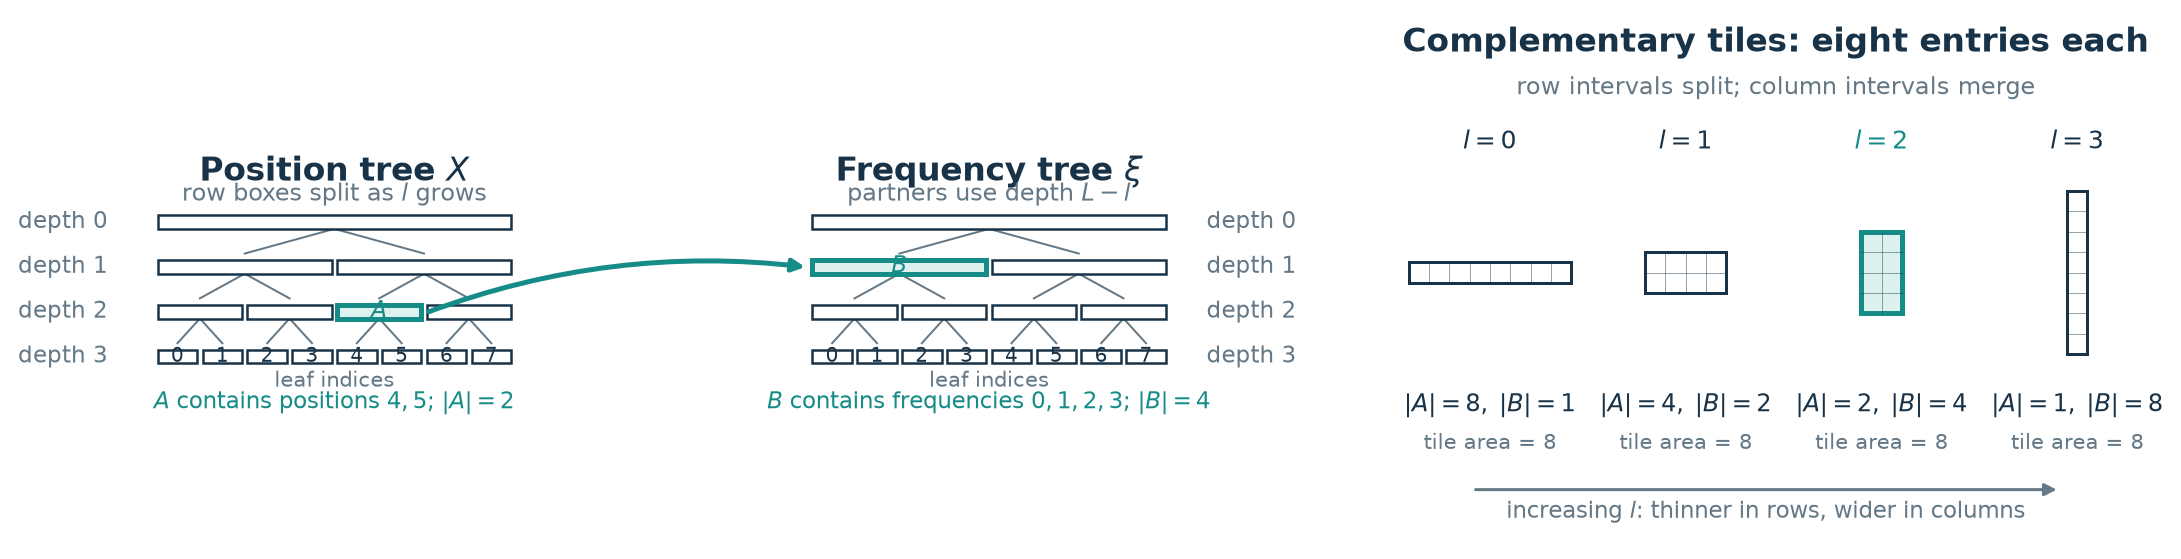
\includegraphics[width=0.94\linewidth]{figures/two-trees.png}
\vspace{1mm}
\begin{columns}[T]
 \column{0.48\textwidth}
 \small
 \textbf{Geometry:} at stage $\ell$, a row node at depth $\ell$ is paired with a column node at depth $L-\ell$. Here $\ell=2$, $L-\ell=1$ and $L=3$.
 \column{0.48\textwidth}
 \small
 \textbf{Cost:} entry area stays fixed, which controls the mixed phase. Independent middle tiles still cost $O(rN^{3/2})$; nested transfers reduce the whole chain to $O(N\log N)$ at bounded ranks.
\end{columns}
\vspace{1mm}
\takeaway{The second tree chooses the tiles; nesting connects their bases.}
\end{frame}

% 7 DFT exact case and solve
\begin{frame}{The same framework explains FFT and a direct solve}
\begin{columns}[T]
 \column{0.48\textwidth}
 \textbf{FFT: ordering makes rank exactly one}
 \small
 For a residue-class tile with $N=2^L$, put
 \[
  j=a+2^\ell u,\qquad k=b+2^{L-\ell}v.
 \]
 Then
 \[
  \frac{jk}{N}=\frac{ab}{N}+\frac{av}{2^\ell}+\frac{bu}{2^{L-\ell}}+\underbrace{uv}_{\in\mathbb Z}.
 \]
 So every tile separates into row and column vectors -- exactly rank one.
 \begin{itemize}
  \item Bit reversal on \textbf{both} trees is essential.
  \item Stored count: $2N\log_2N+2N$.
 \end{itemize}
 \column{0.47\textwidth}
 \textbf{RS/FMM-LU: redundancy enables elimination}
 \small
 Find $A_{F,R}\approx A_{F,S}T$, so a redundant interaction is already described by skeletons. Then eliminate locally:
 \[
  \begin{bmatrix}P&Q\\R&S\end{bmatrix}
  \begin{bmatrix}a\\b\end{bmatrix}
  =\begin{bmatrix}f\\g\end{bmatrix},
 \]
 \[
  (S-RP^{-1}Q)b=g-RP^{-1}f.
 \]
 Repeat through the tree, solve the root, and propagate backwards.
 \vspace{1mm}
 \small This adds stable pivots and modified-block tracking: a solver needs more than an accurate apply.
\end{columns}
\end{frame}

% 7 experiments
\begin{frame}{New problems require additional mathematical structure}
\scriptsize
\begin{columns}[T]
 \column{0.49\textwidth}
 \begin{tabularx}{\linewidth}{@{}c>{\raggedright\arraybackslash}X@{}}
 \textbf{Experiment} & \textbf{Additional structure, and its job}\\
 \midrule
 \textbf{Complex Helmholtz} & Adjoint congruence: keep complex elimination pivots positive, rather than assuming the plain transpose is safe.\\
 \addlinespace[1.4mm]
 \textbf{Stokes flow} & Block-valued sampling: compress Stokes vector components while sharing the tree and solver.\\
 \addlinespace[1.4mm]
 \textbf{Screening/heat} & Absolute/global tolerance for tiny screened blocks; Rothe history for heat time stepping.\\
 \addlinespace[1.4mm]
 \textbf{Fractional/Riesz} & Richer proxy geometry: several latitudes or an annulus, rather than more of the same circle.\\
 \end{tabularx}
 
 \column{0.49\textwidth}
 \begin{tabularx}{\linewidth}{@{}c>{\raggedright\arraybackslash}X@{}}
 \textbf{Experiment} & \textbf{Additional structure, and its job}\\
 \midrule
 \textbf{Volume scattering} & Two-sided contrast handling: the scattering coefficient belongs on the unknown side, not the proxy side.\\
 \addlinespace[1.4mm]
 \textbf{Spherical harmonics} & Two trees + associated-Legendre tiles; Gauss weights give analysis as an exact transpose.\\
 \addlinespace[1.4mm]
 \textbf{Matérn covariance} & Related Matérn kernel orders: supply the boundary information one proxy order misses.\\
 \addlinespace[1.4mm]
 \textbf{Oseen wake} & Directional boxes for the wake, with the total-cost and functional-versus-density distinction.\\
 \end{tabularx}
\end{columns}
\vspace{2mm}
\small Takeaway: each experiment shows which extra mathematical ingredient its problem needs.
\end{frame}

% 8 implementations measured
\begin{frame}{Small problem files, real tested backends}
 \small
 \textbf{Python:} small problem definitions above a shared tree/ID/solver/butterfly driver, ten showcase models and all twelve experiments.

 \textbf{Rust:} a small kernel closure above QR compression, apply and timing; 21 checks plus a separate complex-FIO/recursive-solve prototype.

 \textbf{Both:} independently recover rank-one DFT tiles and the exact count $2N\log_2N+2N$.

\vspace{2mm}
\begin{center}
\small
\begin{tabular}{@{}lrrr@{}}
\toprule
\multicolumn{4}{c}{\textbf{Rust apply at $N=2048$, $\eps=10^{-6}$: same process, not a language race}}\\
Kernel & Storage/dense & Apply error & Apply speedup\\
\midrule
Laplace / log & 0.077 & $2.8\times10^{-7}$ & $11.8\times$\\
Gaussian & 0.058 & $2.8\times10^{-7}$ & $12.6\times$\\
Screened & 0.036 & $1.0\times10^{-15}$ & $14.7\times$\\
\bottomrule
\end{tabular}
\end{center}
\vspace{1mm}
{\footnotesize Compression takes about $0.96$ s at this size (dense-to-compressed oracle); the saving pays after repeated applies.}
\end{frame}

% 9 takeaway
\begin{frame}{What to remember}
\begin{enumerate}
 \item \textbf{Blocks share structure.} Distant or complementary interactions need fewer patterns than the full table.
 \item \textbf{Trees organize where to look.} Weak, strong and complementary blockings answer different geometric questions.
 \item \textbf{Representation and sampling are separate jobs.} What we store is not how we obtain it.
 \item \textbf{Assembly decides the algorithm.} Translate, eliminate, recurse bases, or recombine the FFT.
\end{enumerate}
\vspace{3mm}
\takeaway{One strategy; different mathematics for each problem.\\ Tiles give low rank; nesting gives speed.}
\vspace{3mm}
\small
The report supplies derivations and every experiment; both code packages include reproduction scripts.
\end{frame}

\appendix
% 10: optional definitions
\begin{frame}{Backup: one-minute glossary}
\begin{description}
 \item[Block] A rectangular group of matrix entries sharing a useful structure.
 \item[Low numerical rank] Few patterns approximate a block at specified tolerance.
 \item[ID] Select skeleton columns so other columns can be reconstructed from them.
 \item[Schur complement] What remains after eliminating a group from a linear system.
 \item[Complementary tiling] Finer row groups paired with coarser column groups in two trees.
 \item[Proxy sampling] Auxiliary observations used instead of reading every far interaction.
 \item[$\eps$] Requested relative tolerance; no rank is meaningful without it.
\end{description}
\end{frame}

% 11: optional experiment specifics
\begin{frame}{Backup: three concise checks behind the narrative}
\textbf{DFT tiles, Python and Rust:}
at $N=1024$, every stage rank one and $22{,}528$ stored entries; Rust error $1.83\times10^{-16}$ against a separate FFT.

\vspace{2mm}
\textbf{Reference-core equivalence:}
72/89 golden values exact. The remaining 17 are documented QR-tolerance-boundary rank/count differences, while the measured solver/butterfly errors remain below $10^{-8}$. Portability should be judged through achieved error, not bit-identical rank counts.

\vspace{2mm}
\textbf{Experiment arithmetic:}
Stokes is about $2\times$ per box, $1\times$ per dof and $4\times$ storage at equal geometry. The high-$\lambda$ Oseen root shrinks about $3\times$, but at $N=4096$ the tested directional rule has $-21.6\%$ skeletons for $+28.6\%$ storage and $+67.3\%$ elimination flops. A smaller root is not a total-cost win.
\end{frame}

% 12: pointer to report
\begin{frame}{Backup: where the detailed evidence is}
\begin{itemize}
 \item \textbf{Report:} \texttt{latex/report.tex} and \texttt{main.pdf}: full derivations and algorithm map.
 \item \textbf{Python experiments:} \path{python/unified/explore/e1_*}, ..., \path{e12_*}, each with findings, saved JSON and figures.
 \item \textbf{Rust benchmarks:} \path{rust/results/summary.json}, raw min/median samples and RSS; \path{rust/results/verification-output.txt}.
 \item \textbf{Exact DFT:} \path{rust/results/dft-as-butterfly.txt} and fourteen structural invariants.
 \item \textbf{Cleanup ledger:} \path{python/docs/PROVENANCE.md}; implementation scope: \path{rust/PORT_STATUS.md}.
\end{itemize}
\end{frame}

\end{document}
